% Author: David Larsen <dcl9934@cs.rit.edu>
\listfiles
\documentclass[11pt]{article}
\usepackage{fullpage}
\usepackage{listings}
\usepackage{needspace}
\usepackage{color}
\usepackage{ifthen}
\usepackage{graphicx}
\usepackage{csc}

\lstset{ %
basicstyle=\footnotesize,       % the size of the fonts that are used for the code
numbers=left,                   % where to put the line-numbers
stepnumber=1,                   % the step between two line-numbers. If it's 1 each line will be numbered
numbersep=5pt,                  % how far the line-numbers are from the code
showspaces=false,               % show spaces adding particular underscores
showstringspaces=false,         % underline spaces within strings
tabsize=4,		                % sets default tabsize to 4 spaces
language=Python
}

\ifthenelse{\isundefined{\isAnswerKey}}
{
    \newenvironment{answer}{\large\lstset{basicstyle=\tiny}\color{white}}{}
}
{
    \newenvironment{answer}{\large\lstset{basicstyle=\large}\color{red}}{}
}

\title{CS-141 Midterm Exam Review}
\author{Computer Science Community}
\date{\today}

\makeatletter
\let\thetitle\@title
\let\theauthor\@author
\let\thedate\@date
\makeatother

\begin{document}
\header

\begin{enumerate}
    \item \label{reverse()} Write a recursive function that reverses a string (e.g. ``Don't
        get sick'' yields ``kcis teg t'noD'').

\begin{answer}
\begin{lstlisting}
def reverse( string ):
    if string == '' :
        return string
    else:
        return reverse( string[1:] ) + string[0]
\end{lstlisting}
Other solutions are possible.
\end{answer}

    \item Perform a substitution trace on \texttt{reverse('Doge')}.
%\needspace{15\baselineskip}

\begin{answer}
\begin{lstlisting}[numbers=none]
reverse('Doge')
reverse('oge') + 'D'
reverse('ge') + 'o' + 'D'
reverse('e') + 'g' + 'o' + 'D'
'e' + 'g' + 'o' + 'D'
'egoD'
\end{lstlisting}
\end{answer}

 	\item What does the following evaluate to?
    \begin{lstlisting}
def writeThatDown( n ):
    if n < 5:
        return n
    return (2 * n)

def he( n ):
    temp = n + 180
    if temp > 185:
        return temp
    return n

def putstheFernback( n ):
    return -n

n = 20
n = he(putstheFernback(writeThatDown( n ) ) )
print( n )
    \end{lstlisting}
    \begin{answer}
        -40
    \end{answer}

\pagebreak
    \item Define a function that takes an input string and rotates the sequence
        of letters in each word by n. For example: shift\_left(``DEADBEEF'', 3)
        will produce the output string ``DBEEFDEA''. \\ shift\_left("Giant Robot", 4) will produce "t RobotGian"\\ 
        shift\_left("X", 5) will produce "X" \\You should be able to
        shift a string by a value greater than the length of the
        string\footnote{The modulus (\%) operator, which finds the remainder of a 
        division operation, will be useful here.}.\\ 
        \emph{Assume a function \texttt{len( str )} which returns the length of a string is provided.}

    \begin{enumerate}
        \item Design: Give brief description on how your function should
            accomplish this.

            \begin{answer}
            Our implementation will grab the first part of the new string by
            slicing all characters at an index after the offset. The second
            part of the string will be all of the characters up to the offset
            point. We will then concatenate the two strings.

            Making it possible for the offset to be greater than the length of
            the string can be accomplished by making {\tt offset = offset mod
            len(string)}
            \end{answer}

        \item Testing: Provide 3 test cases, using specific values for the input
            string and amount of shifting and what the expected output should be
            for each.

            \begin{answer}
                shift\_left(``'', 5) should return ""\\
                shift\_left(``A'',5) should return "A"\\
                shift\_left(``ABADCAFE'',300) == shift\_left("ABADCAFE",4)\\
                shift\_left(``FOO'', 1) should return "OOF"
            \end{answer}

        \item Implement the function in Python.

\begin{answer}
\begin{lstlisting}
def shift_left(string, offset):
    if len(string) == 0:
        return string
    else:
        offset = offset % len(string)
        first = string[offset:]
        last = string[:offset]
        return first + last
\end{lstlisting}
\end{answer}

        \item Implement the function {\tt shift\_right()}, which rotates letters
            in the opposite direction.

\begin{answer}
\begin{lstlisting}
def shift_right(string, offset):
    return shift_left(string, -offset)
\end{lstlisting}
\vspace{0.5in}
\end{answer}

    \end{enumerate}


\vfill
\pagebreak

    \item Write a function that takes in a file name, and returns the average size of a word in that file. Assume the files will only have 1 word per line, for example:

        \begin{center}
        No\\
        soup\\
        for\\
        you!
        \end{center}

        which has an average length of: 3.25 \\ \emph{Assume a function \texttt{len( str )} which returns the length of a string is provided.}


\begin{answer}
\begin{lstlisting}
def average_wordlength(filename):
    characters = 0
    words = 0
    for line in open(filename):
        words += 1
        characters += len(line)
    return characters/words
\end{lstlisting}
\end{answer}


    \item Write a function that takes in a string representation of a number and returns the sum
        of all of digits in the string. For example, \texttt{sum( '11111' )} returns 5. \\
        \emph{Assume a function \texttt{len( str )} that returns the length of a string is provided. \\
         Further, assume there is a function \texttt{int( str )} which, given a string representation of an integer, returns its integer value.}

        \begin{enumerate}
            \item Recursively. 
\begin{answer}
\begin{lstlisting}
def sumRec( numbers ):
    if len( numbers ) == 0:
        return 0
    else:
        return int(numbers[0]) + sumRec( numbers[1:] )
\end{lstlisting}
\end{answer}

            \item Iteratively
\begin{answer}
\begin{lstlisting}
def sumIt( numbers ):
    total = 0
    while numbers != '':
        total += int( numbers[0] )
        numbers = numbers[1:]
    return total
\end{lstlisting}
\end{answer}
            \vspace{.25in}
    		\item How would you test this function?
                \begin{answer}
                \begin{itemize}
                    \item Empty string 
                    \item String length = 1
                    \item string length $>$ 1
                \end{itemize}
                \end{answer}
\end{enumerate}

    
\pagebreak
	\item %
% NOTE: This question is meant to take up one full page
%	and includes all necessary spacing.
%


Assuming the turtle is facing East, write the Python code to draw the following picture given the proper depth as input:
    \begin{itemize}
            \item depth = 0
           \\No output 
            \item depth = 1\\
            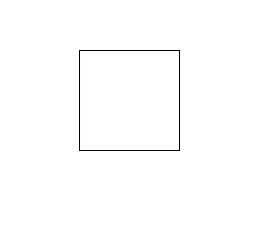
\includegraphics[scale=0.4]{other/1.png}
            \item depth = 2 \\
            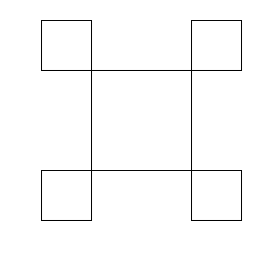
\includegraphics[scale=0.4]{other/2.png}
            \item depth = 3\\
            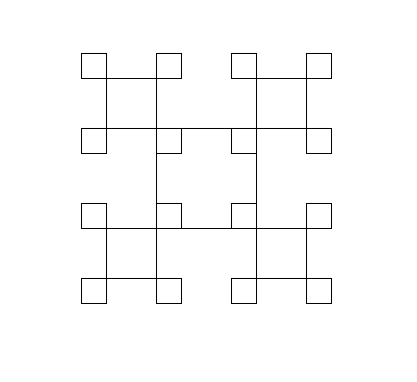
\includegraphics[scale=0.4]{other/3.png}
        \end{itemize}
    \begin{answer}

\vspace{-28pt}

    \begin{lstlisting}
       def drawSqaures( length, depth ):
           if depth <= 0:
               return
           count = 4
           while count > 0:
               turtle.forward( length )
               turtle.left( 90 )
               drawSqaures( length/2, depth-1 )
               turtle.right( 180 )
               count -= 1
      \end{lstlisting}
        NOTE: Solution starts from top-left corner of the main box.
     \end{answer}



\newpage
	\item Connor is a big dweeb and loves keeping a count of things.
You will be writing a tail-recursive function to satisfy his desires.
\begin{enumerate}

\item
\label{tailrecursive}
Write a tail recursive function \texttt{coRec}, which takes a string and a character and returns the number of times the character appears in the string. \\
For example, \texttt{coRec("Eric is enjoying the weather.", 'i')} should return \texttt{3}. \\
Do not use the \texttt{len()} function.
\begin{answer}
\begin{lstlisting}
def coRec(string,char,counter=0):
    if(string==''):
        return counter
    if(strHead(string)==char):
        return coRec(strTail(string),char,counter+1)
    else:
        return coRec(strTail(string),char,counter)
\end{lstlisting}
\end{answer}

\item
What is the complexity of the functions you wrote for \ref{tailrecursive}?
\begin{answer}

It runs in O(N) time. \\
\end{answer}
\end{enumerate}


	\item Write a function which performs basic string compression, using the counts of repeated characters. For example, 
the string $abbbccccaaa$ would be compressed to: $a1b3c4a3$. \\
 \emph{Assume the function \texttt{len( str )}, which returns the length of a string, is provided. \\
      Further, assume you may use \texttt{int( str )} and \texttt{str( int )}, which converts a string to its integer representation, and converts an integer to its string representation, respectively.}

\begin{answer}
\begin{lstlisting}
def compress( string ):
    new = ''
    curChar = string[0]
    count = 0
    for char in string:
        if char == curChar:
            count += 1
        else:
            new = new + curChar + str(count)
            curChar = char
            count = 1 

    new = new + curChar + str(count)
    return new
\end{lstlisting}
\end{answer}


\newpage
	\item How can you use a stack to check if an input string
of exclusively parentheses, brackets, and braces is properly balanced?
(e.g. ``[\{\}]'' is accepted, but ``(()'' and ``[(])'' are not.)\\
Assume that you are provided with a \texttt{Stack} class that has \texttt{push()}, \texttt{pop()}, and \texttt{peek()} member functions.

\begin{answer}
\begin{lstlisting}
def closing_match(char):
	if char == '(':
		return ')'
	elif char == '[':
		return ']'
	elif char == '{':
		return '}'
	elif char == '<':
		return '>'
	else:
		return None

def delims_are_balanced(inString):
    ''' String -> boolean
    Determines if the input string has balanced delimiters.
    Delimiters are () [] {} and <>.
    
    '''
    stack = Stack()
    for char in inString:
        if closing_match(char) != None: # a starting grouping symbol
            stack.push(char)
		else:
			if stack.is_empty():
				return False
			elif char == closing_match(stack.peek()):
				stack.pop()
			else: # mismatched grouping symbol
				return False
    return stack.is_empty()
\end{lstlisting}
\end{answer}
\vspace{1.5in}

\newpage
	\item %
% NOTE: This question is meant to take up one full page
%	and includes all necessary spacing.
%


Sally is being plagued by an army of lookalike suiters, each of which presents her with an enticing but unbearable meal upon arrival.
The dishes all smell amazing, however, so she can't help but try each one.
A dish will never fail to disappoint her, but fortunately, some of the suiters shared recipes and created identical concoctions.
Once Sally tastes a meal once, she can immediately smell out instances of the same dish and send their bearers away.
\begin{enumerate}
\item
\label{listdupes}
Write a Python function that, given a list of ``dishes,'' returns a list of the rejected dishes in the order they failed to fool her. (e.g. $[1, 2, 2, 3, 3, 3]$ would return [2,3,3] )
\begin{answer}
\begin{lstlisting}
def find_dupes(lst):
	result=[]
	seen=[]
	for member in lst:
		if member not in seen:
			seen.append(member)
		else:
			result.append(member)
	return result
\end{lstlisting}
\end{answer}

\item
If your solution to \ref{listdupes} was iterative, write it recursively; if it was recursive, write it iteratively.
\begin{answer}
\begin{lstlisting}
def find_recur(lst, seen=[]):
	if len(lst)==0:
		return []
	if lst[0] not in seen:
		seen.append(lst[0])
		return find_recur(lst[1:], seen)
	return [lst[0]]+find_recur(lst[1:], seen)
\end{lstlisting}
\textit{or}
\begin{lstlisting}
def find_tail(lst, result=[], seen=[]):
	if len(lst)==0:
		return result
	if lst[0] not in seen:
		seen.append(lst[0])
	else:
		result.append(lst[0])
	return find_tail(lst[1:], result, seen)
\end{lstlisting}
\end{answer}

\item
What is the time complexity of your approach?
Why? \\

\begin{answer}
$O(N^2)$, since the \texttt{seen} list must be searched linearly
\end{answer}
\end{enumerate}

\newpage
	\item For the sake of this question, you find yourself to be the head programmer under Kim Jong Un's glorious reign.
It also just so happens that a nation-wide track meet is being held today. Thus, the glorious leader has demanded that
you write a program to keep track of information relating to all track runners present at the event.

\begin{enumerate}
\item Write a class named \texttt{TrackRunner} to keep track of all runners competing.
You will need to store their \texttt{name}, \texttt{age}, and \texttt{fastestTime}.
\begin{answer}
\begin{lstlisting}
class TrackRunner:
    __slots__=('name','age','fastestTime')

\end{lstlisting}
\end{answer}

\item Now write a function to make an individual \texttt{TrackRunner} object.
\begin{answer}
\begin{lstlisting}
def makeRunner(r_name,r_age,r_fastestTime):
    runner = TrackRunner()
    runner.name = r_name
    runner.age = r_age
    runner.fastestTime = r_fastestTime
    return runner
\end{lstlisting}
\end{answer}

\item The glorious leader has decided that, on this day, no runner named \texttt{Joe} may win
gold. Given a list of \texttt{TrackRunner} objects, write the function \texttt{aWinnerIsYou(r)} that finds the runner in the list \texttt{r} with the fastest time who's name is not "Joe". 
Then print the runner's name, age and time.
\begin{lstlisting}

\end{lstlisting}
\begin{answer}
\begin{lstlisting}
def aWinnerIsYou(r):
    best = None
    for i in range(len(r)):
        if r[i].name != 'Joe':
            if best == None:
                best = r[i]
            elif best.fastestTime > r[i].fastestTime:
                best = r[i]
    return best

best = aWinnerIsYou(runnersLst)
print(best.name, best.age, best.fastestTime)
\end{lstlisting}
\end{answer}
\end{enumerate}


\newpage

	\item Below is Python code for a function that performs an insertion sort
    and prints \texttt{data} after each iteration of the \texttt{for} loop.
\begin{lstlisting}
def insertion_sort( data ):
    for marker in range( 1, len( data ) ):
        val = data[marker]
        i = marker
        while i > 0 and data[i-1] > val:
            data[i] = data[i-1]
            i -= 1
        data[i] = val
        print( data )
\end{lstlisting}
\begin{enumerate}
\item
Write out what the function will print for the input list: [3,2,7,1].
\begin{answer}
\begin{lstlisting}
[2,3,7,1]
[2,3,7,1]
[1,2,3,7]
\end{lstlisting}
\end{answer}

\item What is the sort algorithm's time complexity?
\begin{answer}

O(N\textsuperscript{2})
\end{answer}
\end{enumerate}

	\item \textbf{Greedy algorithms.}
In the game Black and White\footnote{Special thanks to Professor Butler for unwittingly allowing us to rip off his problem.}, the player is faced with a row of identical double-sided chips.
You can probably guess what colors the two sides of each chip are.
The objective is to flip as many chips as necessary so their exposed colors match that of a target pattern. \\
The catch?
Reordering the chips is said to be Impossible by those who seem to know what they're talking about. \\
The \textit{real} catch?
Flipping a group of consecutive tiles can be accomplished in a single ``action.'' \\
If every flip takes one ``action,'' write a function \texttt{bwMoves} that, given a starting pattern and target pattern as equal-length strings, returns the minimum number of actions required to get them to match.
For instance, \texttt{bwMoves( 'BBWBBWBBBB', 'WWWWWBBWWB' )} should return 3.
\vspace{6pt} \\
\textit{Hint: Were any of the other questions labeled with the concept they were testing?}
\begin{answer}
\begin{lstlisting}
def bwMoves(start, target):
	actions=0
	first=0
	for index in range(len(start)):
		if start[index]==target[index]:
			if first!=index: # Each flip works up to (but not including)
				actions+=1	 # the index pointer. If first==index, that's
			first=index+1	 # 0 elements, so there is nothing to flip.
							 # (i.e. There were two no-flips in a row.)
	if start[-1]!=target[-1]:
		actions+=1
	return actions
\end{lstlisting}
\end{answer}

\end{enumerate}
\end{document}
